\documentclass{ccuthesis}
% 預設 onehalfspacing 1.5行距,可改為 single spacing 或 doublespacing

\university{國立中正大學}
\college{電機工程研究所}
\type{碩士論文}    % 如為初稿,請加上(初稿)
\title{論文名稱}{Thesis Title}
\author{某某某}
\advisor{指導教授:某某某 博士}
\defensedate{中華民國 一百一十四 年 七 月}

% ============================================================================
\begin{document}

% 首頁
\makecover

\pagenumbering{roman}
% 審定書
\clearpage
\begin{center}

\includegraphics[width=\textwidth]{certification example.pdf}  %更改為審定書掃描檔
\end{center}

\clearpage
\addcontentsline{toc}{section}{誌謝}
\section*{誌謝}
% =====在此填入誌謝內容=====
誌謝內文



\clearpage
\addcontentsline{toc}{section}{摘要}
\section*{摘要}
% =====在此填入摘要=====
摘要內文


\medskip\textbf{關鍵字:}關鍵字1、關鍵字2、關鍵字3、關鍵字4、關鍵字5



\clearpage
\addcontentsline{toc}{section}{Abstract}
\section*{Abstract}
% =====在此填入Abstract=====
Abstract content


\medskip\textbf{Keywords:} keyword1, keyword2, keyword3, keyword4, keyword5



\clearpage
\addcontentsline{toc}{section}{目錄}
\tableofcontents  % 目錄
\addtocontents{toc}{\protect{\pdfbookmark[0]{\contentsname}{toc}}} %把目錄頁加入pdf書籤
\clearpage
\addcontentsline{toc}{section}{圖目錄}
\listoffigures  % 圖目錄
\clearpage
\addcontentsline{toc}{section}{表目錄}
\listoftables   % 表目錄
\clearpage

\pagenumbering{arabic}
% ================================論文正文================================

\section{緒論}
\subsection{研究動機}
引用論文時請用 \cite{Rowe:2005:ASR}。若要引用多篇論文,請用 \cite{Rowe:2005:ASR,vinet1989universal}。如插入圖表,請參考圖 \ref{fig:example} 與表 \ref{tab:example}。

\begin{figure}[htbp]
\centering
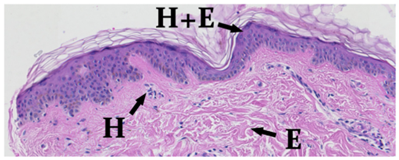
\includegraphics[width=0.7\textwidth]{figures/example.png}
\caption{圖片範例}
\label{fig:example}
\end{figure}

\begin{table}[htbp]
\centering
\caption{表格範例}
\label{tab:example}
\begin{tabular}{cc}
	\toprule
	\textbf{A} & \textbf{B} \\
	\midrule
	1 & 2 \\
	3 & 4 \\
	\bottomrule
\end{tabular}
\end{table}

\subsection{研究目的}
\subsection{研究貢獻}
\subsection{論文架構}

\section{研究背景}
\subsection{相關文獻探討}

\section{研究方法}
\subsection{架構流程}
\subsection{資料集介紹}
\subsection{評估指標}
\subsection{硬體軟體設備}

\section{實驗結果與討論}
\subsection{相關文獻之比較}

\section{結論與未來展望}
\subsection{結論}
\subsection{未來展望}


%% 參考文獻
\clearpage
\bibliographystyle{IEEEtran}
\bibliography{thesis.bib}

\end{document}
